\documentclass[a4paper,11pt]{jsarticle}

% パッケージ
\usepackage[dvipdfmx]{hyperref}
\usepackage{pxjahyper}
\usepackage[dvipdfmx]{graphicx}
\usepackage{ascmac}
\usepackage{fancybox}
\usepackage{listings}
\usepackage{plistings}
\usepackage{multirow}
\usepackage[subrefformat=parens]{subcaption}
\usepackage{color}
\usepackage{here}
\usepackage{amsmath,amsfonts}
\usepackage[utf8]{inputenc}
\usepackage{subcaption}
\usepackage{bm}
\usepackage{siunitx}
\usepackage{url}
% ページの周りの余白
\usepackage[top=25truemm,bottom=25truemm,left=30truemm,right=30truemm]{geometry}

% URLの設定
\Urlmuskip=0mu  plus 10mu

% 色の定義
\definecolor{OliveGreen}{rgb}{0.0,0.6,0.0}
\definecolor{Magenta}{cmyk}{0, 1, 0, 0}
\definecolor{colFunc}{rgb}{1,0.07,0.54}
\definecolor{CadetBlue}{cmyk}{0.62,0.57,0.23,0}
\definecolor{Brown}{cmyk}{0,0.81,1,0.60}
\definecolor{colID}{rgb}{0.63,0.44,0}


\lstset{
  basicstyle={\ttfamily},
  identifierstyle={\small},
  commentstyle={\smallitshape},
  keywordstyle={\small\bfseries},
  ndkeywordstyle={\small},
  stringstyle={\small\ttfamily},
  frame={tb},
  breaklines=true,
  columns=[l]{fullflexible},
  numbers=left,
  xrightmargin=0zw,
  xleftmargin=3zw,
  numberstyle={\scriptsize},
  stepnumber=1,
  numbersep=1zw,
  lineskip=-0.5ex
}

\renewcommand{\lstlistingname}{Code}

% リンクの設定
\hypersetup{
  setpagesize=false,
  bookmarksnumbered=true,
  bookmarksopen=true,
  colorlinks=true,
  linkcolor=blue,
  citecolor=red,
}

\begin{document}

\section{目的}
タランジスタの増幅回路において,最大の無歪み交流出力電あるを得るために,CR結合増幅回路を
作成して入出力交流特性の測定を行う.
\section{実験環境}
以下の表\ref{T:EM}に使用した実験機器を示す.
\begin{table}[H]
  \begin{center}
    \caption{使用した実験機器}
    \begin{tabular}{|c|c|} \hline
      機器                       & 型番,実測値                                    \\ \hline
      LCRメータ                  & HIOKI DMT TDB-401 CI-TEST-16                    \\ \hline
      ブレッドボード             & Sunhayato modelSAD-12                           \\ \hline
      直流定電圧電源             & KIKUSUI ELECTRONIS CORP B123-153                \\ \hline
      直流電流系                 & YES1991 No.71BA00214 YOKOGAWA 8番               \\ \hline
      直流電圧系                 & YES1991 No.71BA00214 YOKOGAWA 10番              \\ \hline
      ディジタルマルチメータ     & ADCMT 7461A Digital Multi meter 22番            \\ \hline
      ファンクションジェネレータ & TEXIO SYNTHESIZED FUNCTION GENERATOR FG-274 6番 \\ \hline
      2現象オシロスコープ        & \begin{tabular}{c}Tektronix TDS 1001B TWO CHANNEL DIGITAL \\ STORAGE OSCILLOSCOPE 40MHz 500 MS/s \end{tabular}                       \\ \hline
      バイアス抵抗               & $1.00\si{\kilo \ohm}$                           \\ \hline
      ブリータ抵抗               & $100\si{\kilo \ohm} (可変)$                     \\ \hline
      エミッタ抵抗               & $1.00\si{\kilo \ohm}$                           \\ \hline
      結合コンデンサ             & $2.208\si{\mu F}, 2.117\si{\mu F}$              \\ \hline
      バイパスコンデンサ         & $98.82\si{\mu F }$                              \\ \hline
      負荷抵抗                   & $1.497\si{\kilo \ohm}, 2.98\si{\kilo \ohm}$     \\ \hline
      コレクタ抵抗               & $3.6\si{\kilo \ohm}$                            \\ \hline
      トランジスタ               & 2SC1815                                         \\ \hline
    \end{tabular}
    \label{T:EM}
  \end{center}
\end{table}
\section{実験方法}
実験資料~\cite{text}に従って実験を行う.
\section{実験結果}
以下に実験から得られたデータを以下の表\ref{T:result}と図\ref{G:result}に示す.
\begin{table}[H]
  \begin{center}
    \caption{実験結果}
    \begin{tabular}{|c|c|c|c|c|c|c|c|} \hline
      \multicolumn{4}{|c|}{$RL = 1.5 \si{\kilo \ohm}$} & \multicolumn{4}{|c|}{$RL = 3 \si{\kilo \ohm}$}                                                       \\ \hline
      \begin{tabular}{c}
        Vi \\
        $[\si{\milli \volt}]$
      \end{tabular}                        &
      \begin{tabular}{c}
        Vo \\
        $[\si{\volt}]$
      \end{tabular}                        &
      \begin{tabular}{c}
        Av \\
        算出値
      \end{tabular}                        &
      \begin{tabular}{c}
        Av \\
        理論値
      \end{tabular}                        &
      \begin{tabular}{c}
        Vi \\
        $[\si{\milli \volt}]$
      \end{tabular}                        &
      \begin{tabular}{c}
        Vo \\
        $[\si{\volt}]$
      \end{tabular}                        &
      \begin{tabular}{c}
        Av \\
        算出値
      \end{tabular}                        &
      \begin{tabular}{c}
        Av \\
        理論値
      \end{tabular}                                                                                                                               \\ \hline
      10                                               & 0.7330                                         & 73.3  & -85.40 & 10.01  & 1.1394 & 113.83 & -131.69 \\ \hline
      20.03                                            & 1.397                                          & 69.75 & -85.40 & 20.00  & 1.970  & 98.50  & -131.69 \\ \hline
      30.05                                            & 1.777                                          & 59.13 & -85.40 & 30.06  & 2.443  & 81.27  & -131.69 \\ \hline
      40.00                                            & 2.013                                          & 50.33 & -85.40 & 40.02  & 2.729  & 68.19  & -131.69 \\ \hline
      50.00                                            & 2.169                                          & 43.38 & -85.40 & 50.04  & 2.908  & 58.11  & -131.69 \\ \hline
      60.07                                            & 2.276                                          & 37.89 & -85.40 & 60.00  & 3.022  & 50.37  & -131.69 \\ \hline
      70.03                                            & 2.352                                          & 33.59 & -85.40 & 70.06  & 3.100  & 44.25  & -131.69 \\ \hline
      80.01                                            & 2.410                                          & 30.12 & -85.40 & 80.00  & 3.155  & 39.44  & -131.69 \\ \hline
      90.06                                            & 4.455                                          & 49.47 & -85.40 & 90.08  & 3.196  & 35.48  & -131.69 \\ \hline
      100.04                                           & 2.490                                          & 24.89 & -85.40 & 100.03 & 3.184  & 31.83  & -131.69 \\ \hline
    \end{tabular}
    \label{T:result}
  \end{center}
\end{table}
\begin{figure}[H]
  \begin{tabular}{cc}
    \begin{minipage}[t]{0.48\textwidth}
      \centering
      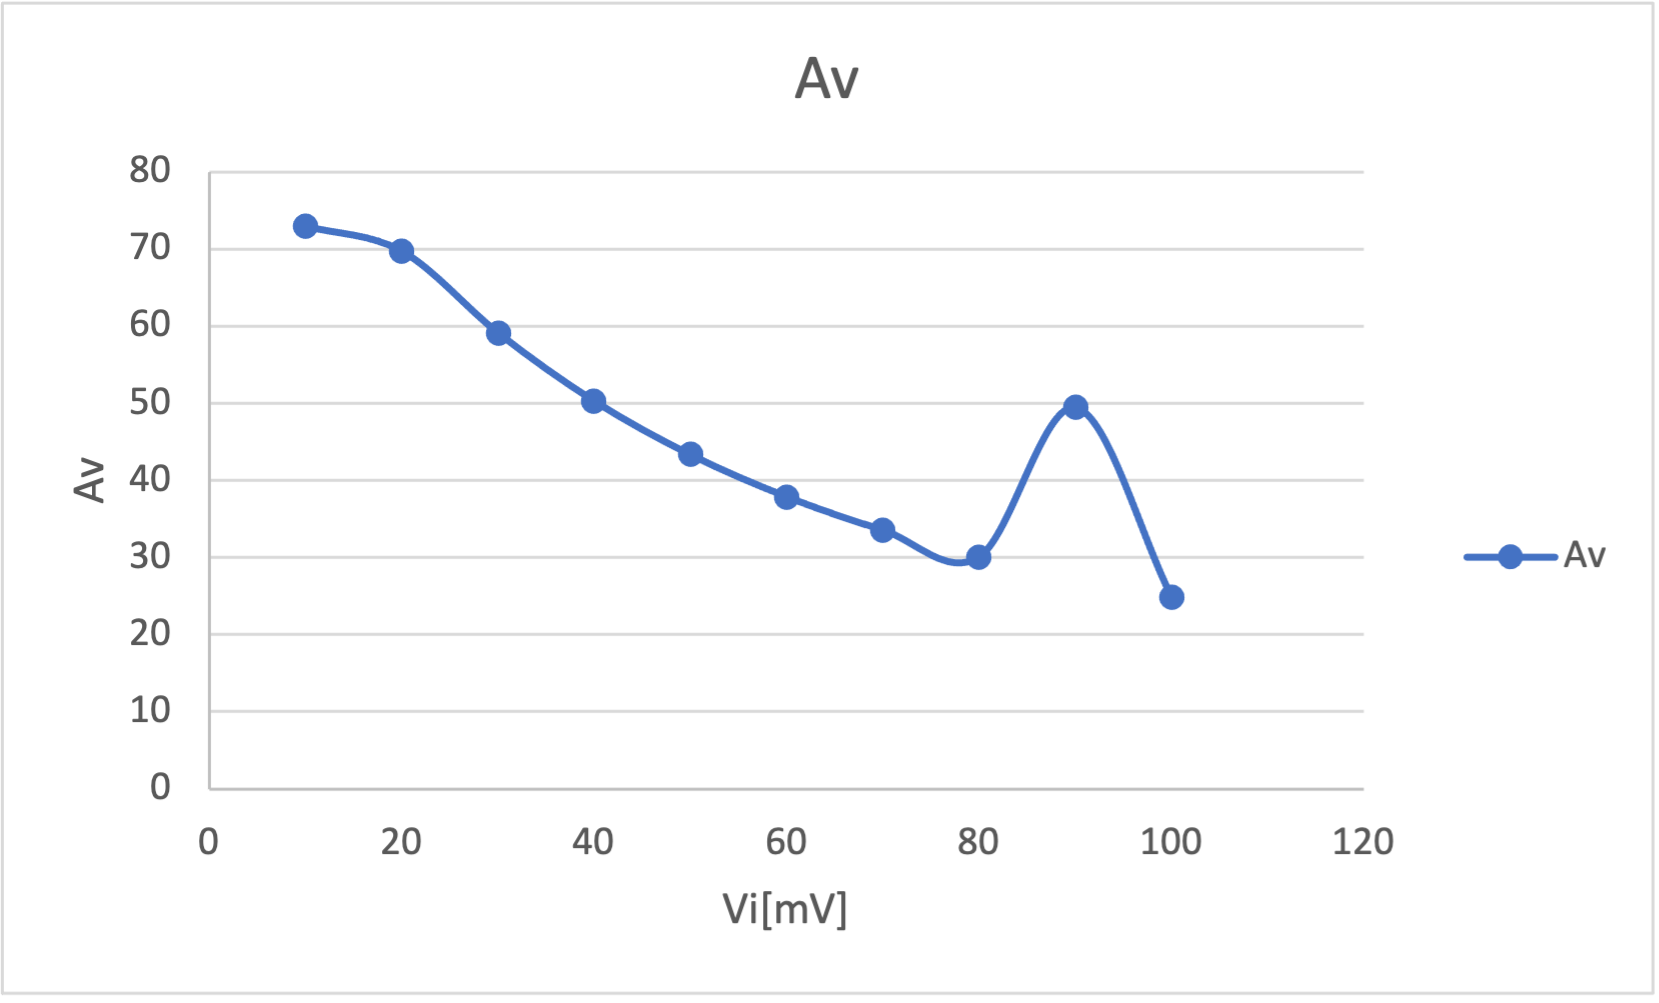
\includegraphics[clip,width=7.6cm]{picture/Av1_5.png}
      \subcaption{RL=1.5$\si{\kilo \ohm}$のときのAv}
      \label{G:1_5Av}
    \end{minipage} &
    \begin{minipage}[t]{0.48\textwidth}
      \centering
      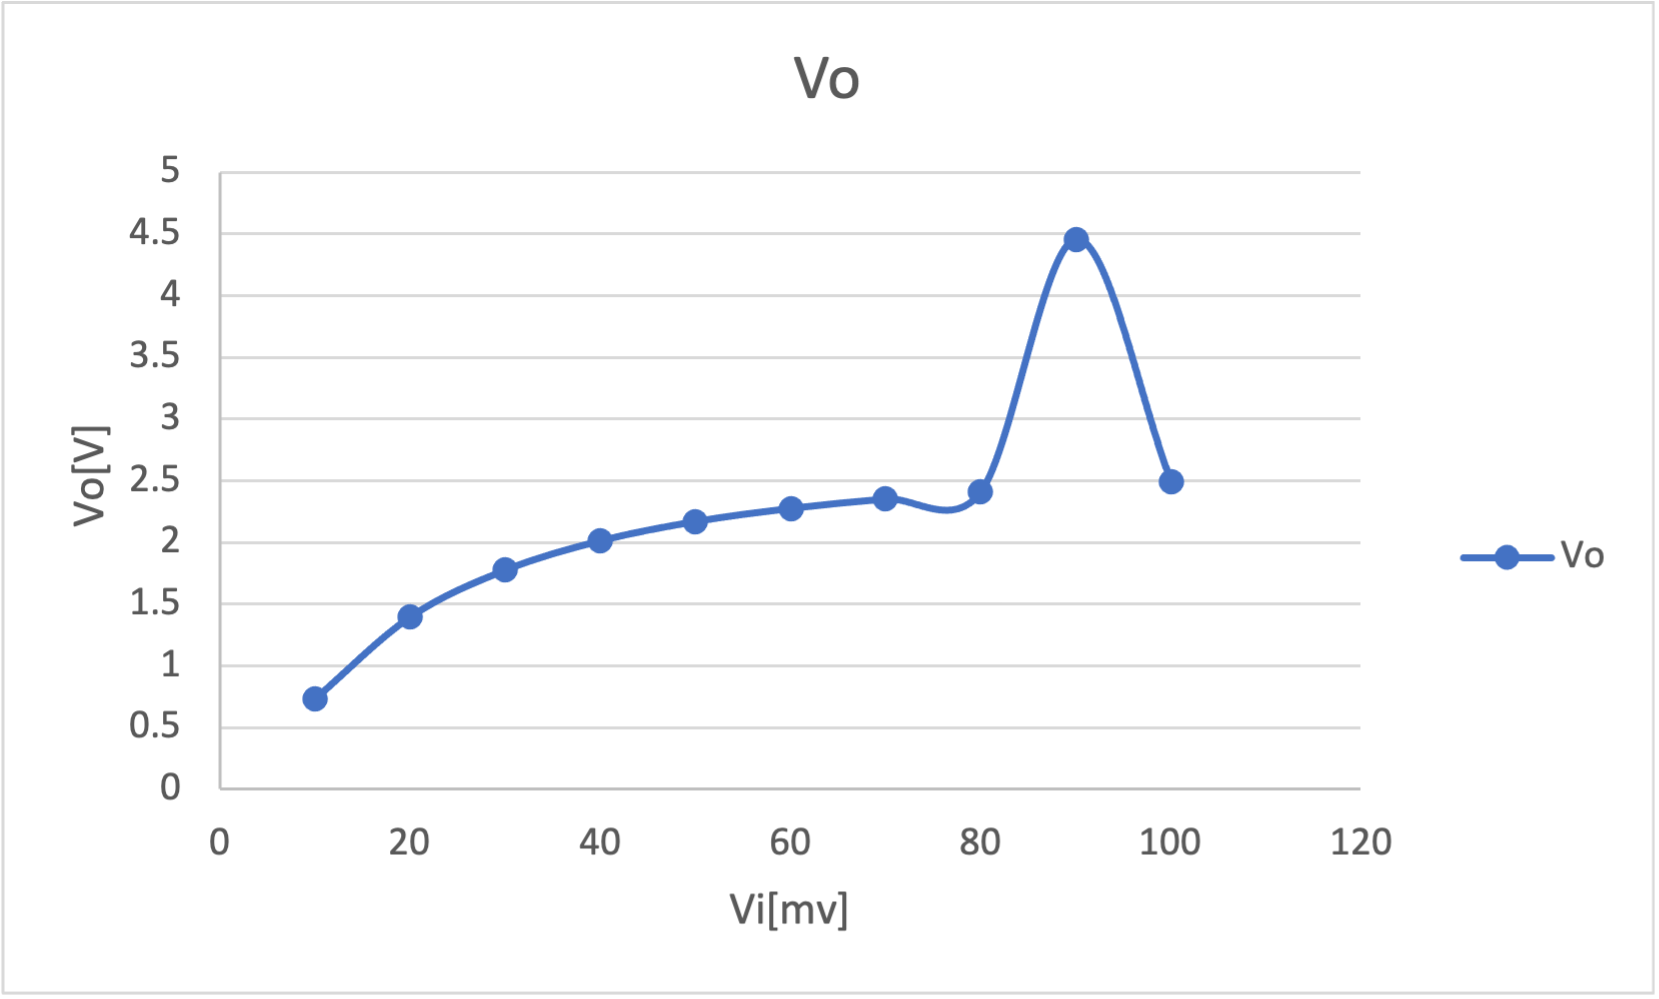
\includegraphics[clip,width=7.6cm]{picture/vo1_5.png}
      \subcaption{RL=1.5$\si{\kilo \ohm}$のときのVo}
      \label{G:1_5Vo}
    \end{minipage}
  \end{tabular}
\end{figure}
\begin{figure}[H]
  \begin{tabular}{cc}
    \begin{minipage}[t]{0.48\textwidth}
      \centering
      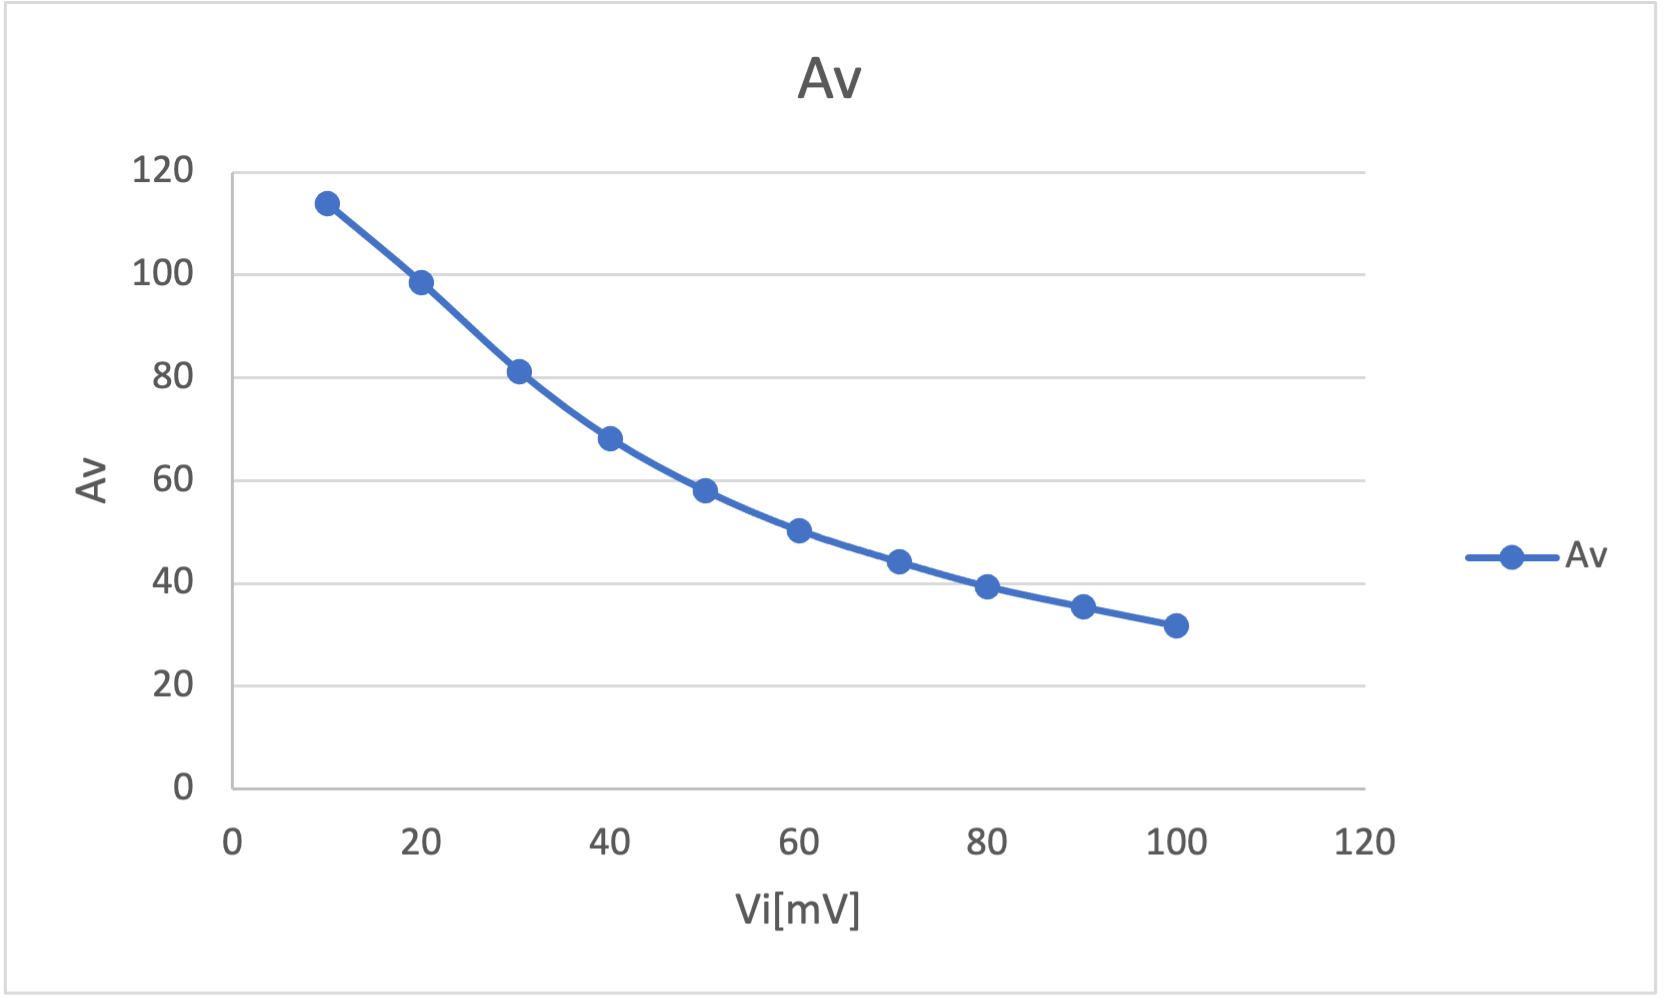
\includegraphics[clip,width=7.6cm]{picture/Av3.png}
      \subcaption{$RL=3\si{\kilo \ohm}$のときのAv}
      \label{G:3Av}
    \end{minipage} &
    \begin{minipage}[t]{0.48\textwidth}
      \centering
      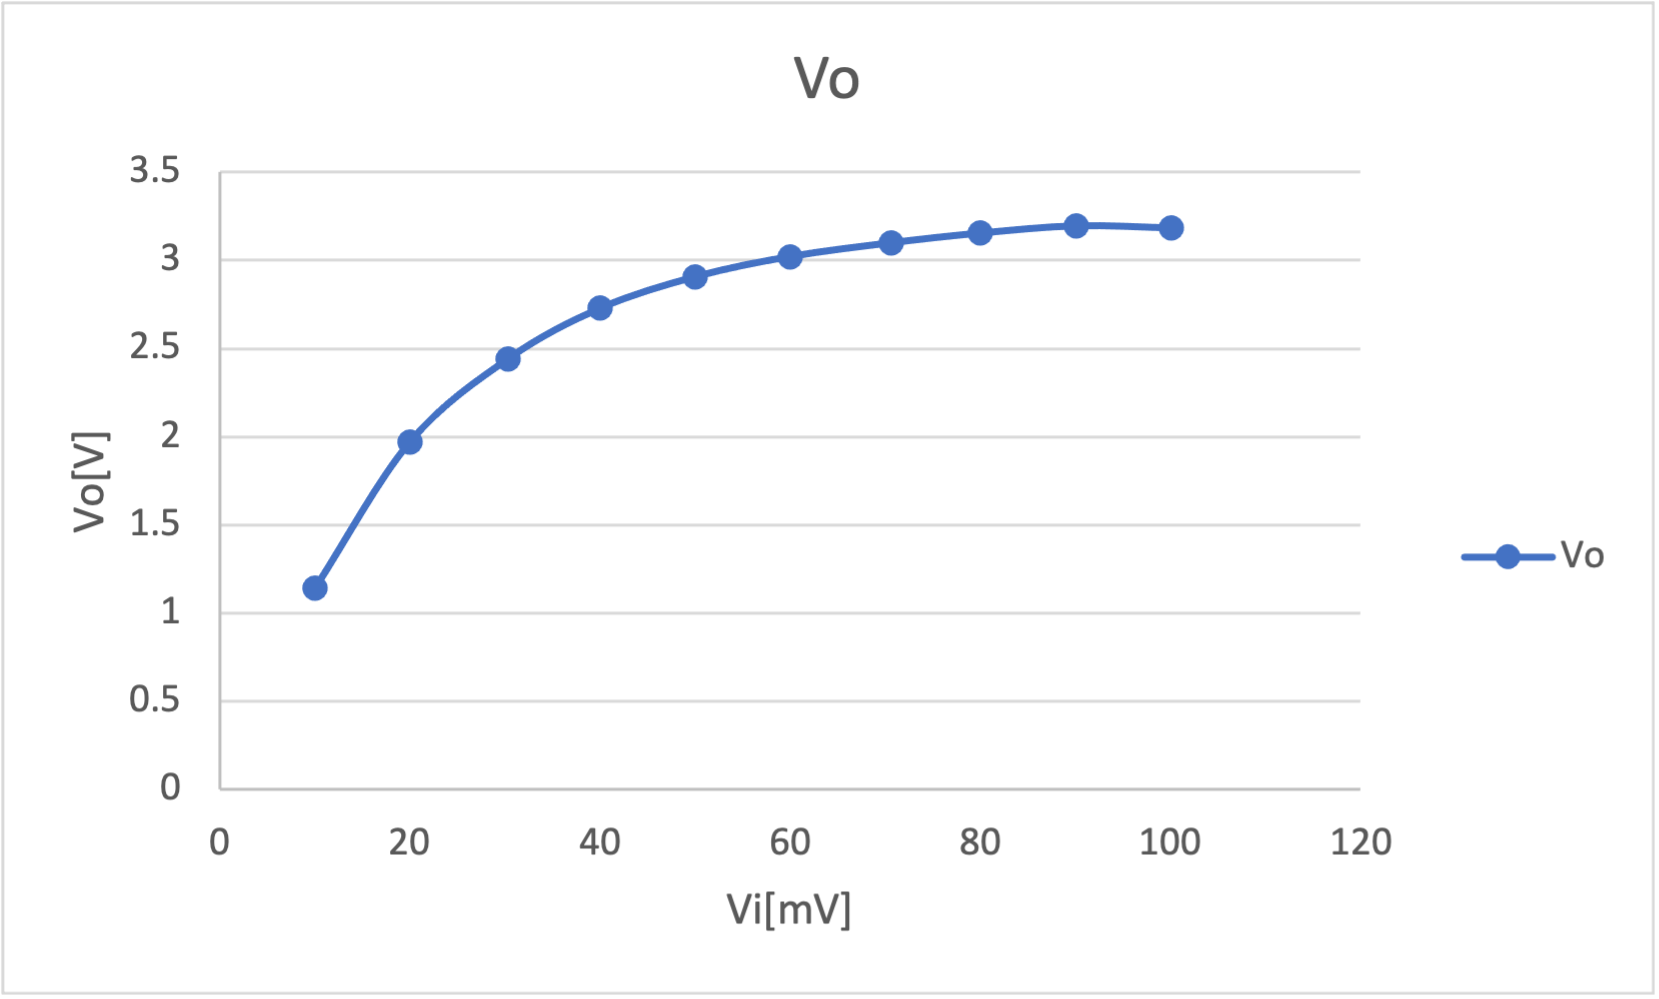
\includegraphics[clip,width=7.6cm]{picture/vo3.png}
      \subcaption{$RL=3\si{\kilo \ohm}$のときのVo}
      \label{G:3Vo}
    \end{minipage}
  \end{tabular}
  \caption{実行結果}
  \label{G:result}
\end{figure}
また,以下の図\ref{G:1_5Scope},\ref{G:3Scope}にオシロスコープで観測した入出力電圧波形を示す.
\begin{figure}[H]
  \begin{center}
    \begin{minipage}{0.48\textwidth}
      \begin{center}
        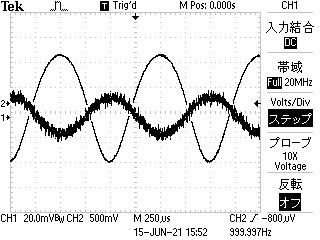
\includegraphics[clip,width=5.8cm]{picture/1.5K_data/TEK0000.jpeg}
      \end{center}
      \subcaption{正弦波形に歪みがない状態}
    \end{minipage}
    \begin{minipage}{0.48\textwidth}
      \begin{center}
        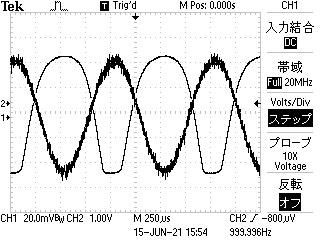
\includegraphics[clip,width=5.8cm]{picture/1.5K_data/TEK0002.jpeg}
      \end{center}
      \subcaption{正弦波形に歪みが出始めた状態}
    \end{minipage} \\
    \begin{minipage}{0.48\textwidth}
      \begin{center}
        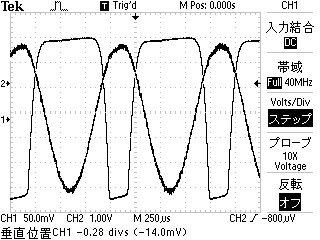
\includegraphics[clip,width=5.8cm]{picture/1.5K_data/TEK0009.jpeg}
      \end{center}
      \subcaption{正弦波形が崩れた状態}
    \end{minipage}
    \caption{$RL=1.5\si{\kilo \ohm}$の出力波形}
    \label{G:1_5Scope}
  \end{center}
\end{figure}

\begin{figure}[H]
  \begin{center}
    \begin{minipage}{0.48\textwidth}
      \begin{center}
        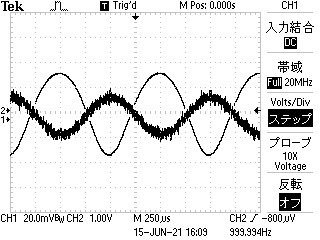
\includegraphics[clip,width=5.8cm]{picture/3K_data/TEK0000.jpeg}
      \end{center}
      \subcaption{正弦波形に歪みがない状態}
    \end{minipage}
    \begin{minipage}{0.48\textwidth}
      \begin{center}
        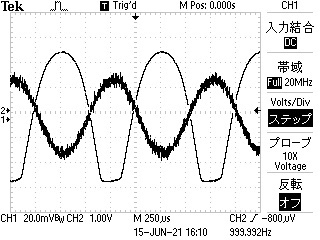
\includegraphics[clip,width=5.8cm]{picture/3K_data/TEK0001.jpeg}
      \end{center}
      \subcaption{正弦波形に歪みが出始めた状態}
    \end{minipage} \\
    \begin{minipage}{0.48\textwidth}
      \begin{center}
        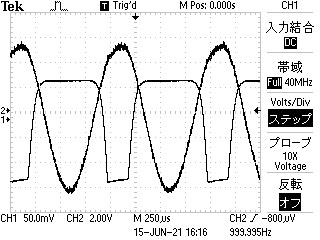
\includegraphics[clip,width=5.8cm]{picture/3K_data/TEK0009.jpeg}
      \end{center}
      \subcaption{正弦波形が崩れた状態}
    \end{minipage}
    \caption{$RL=3\si{\kilo \ohm}$の出力波形}
    \label{G:3Scope}
  \end{center}
\end{figure}

\section{考察}
本実験の図\ref{G:1_5Scope},\ref{G:3Scope}において,グラフに歪みが見られた.この歪みの原因について
考察する.以下の図\ref{G:hukasen}に負荷線を示す.
\begin{figure}[H]
  \begin{minipage}{0.48\textwidth}
    \begin{center}
      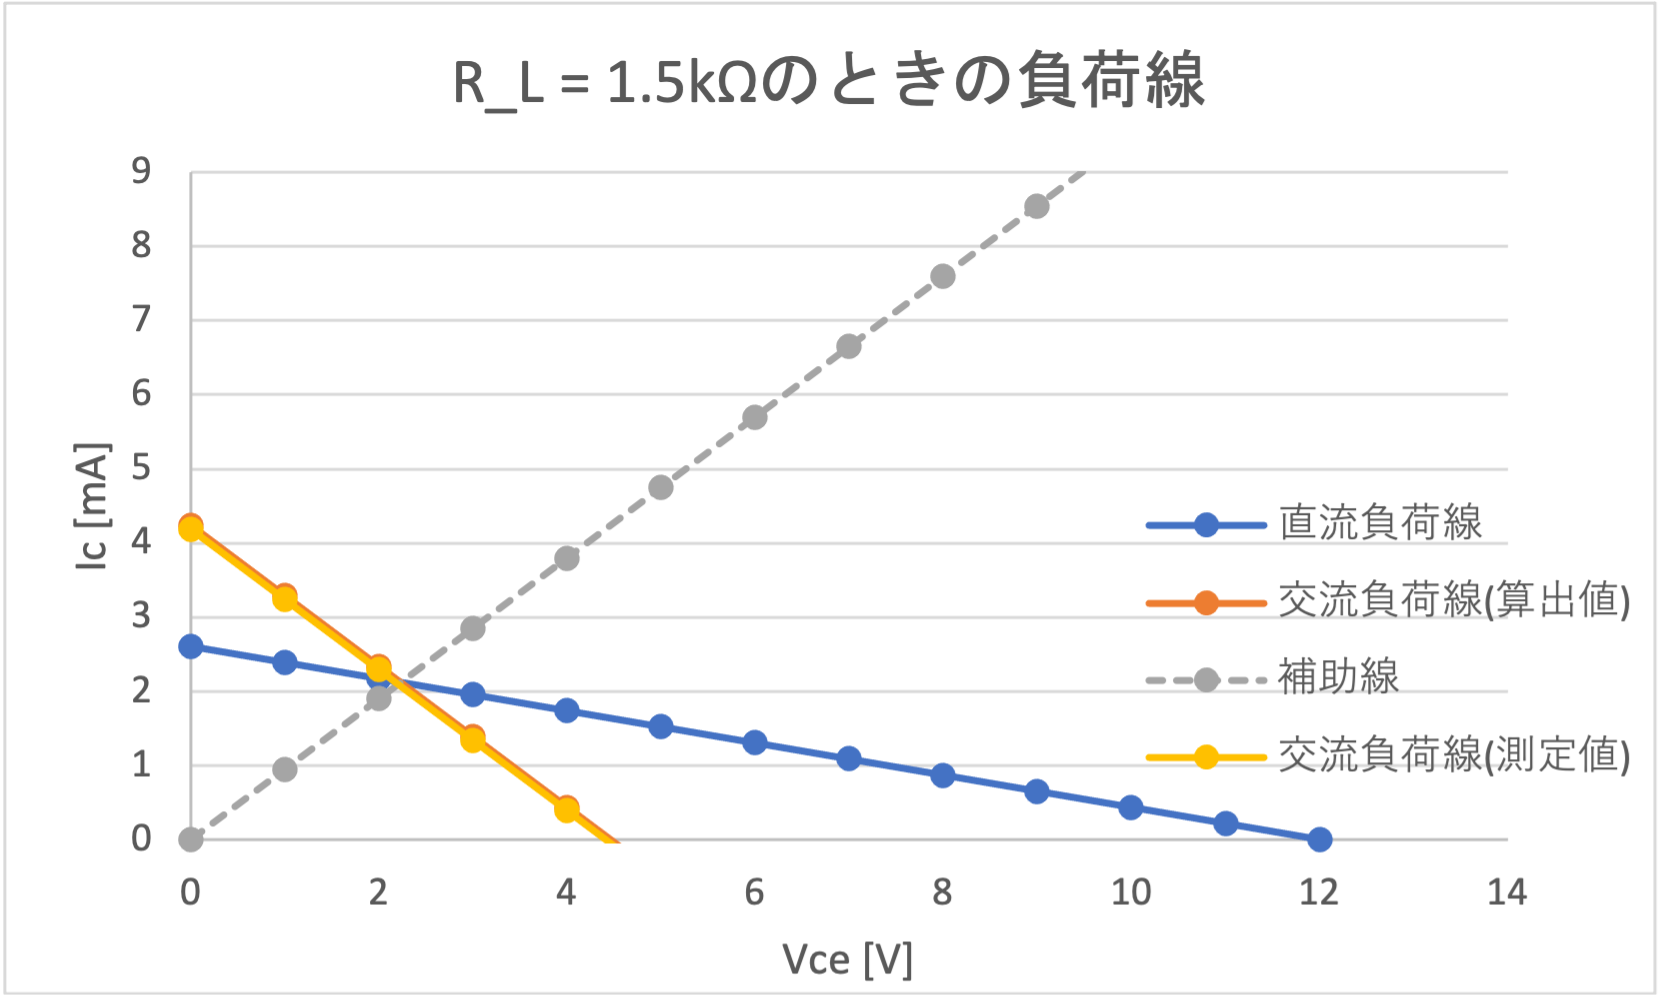
\includegraphics[clip,width=7.5cm]{picture/G1_5.png}
    \end{center}
    \subcaption{$R_L=1.5\si{\kilo \ohm}$のときの負荷線}
    \label{G:1_5huka}
  \end{minipage}
  \begin{minipage}{0.48\textwidth}
    \begin{center}
      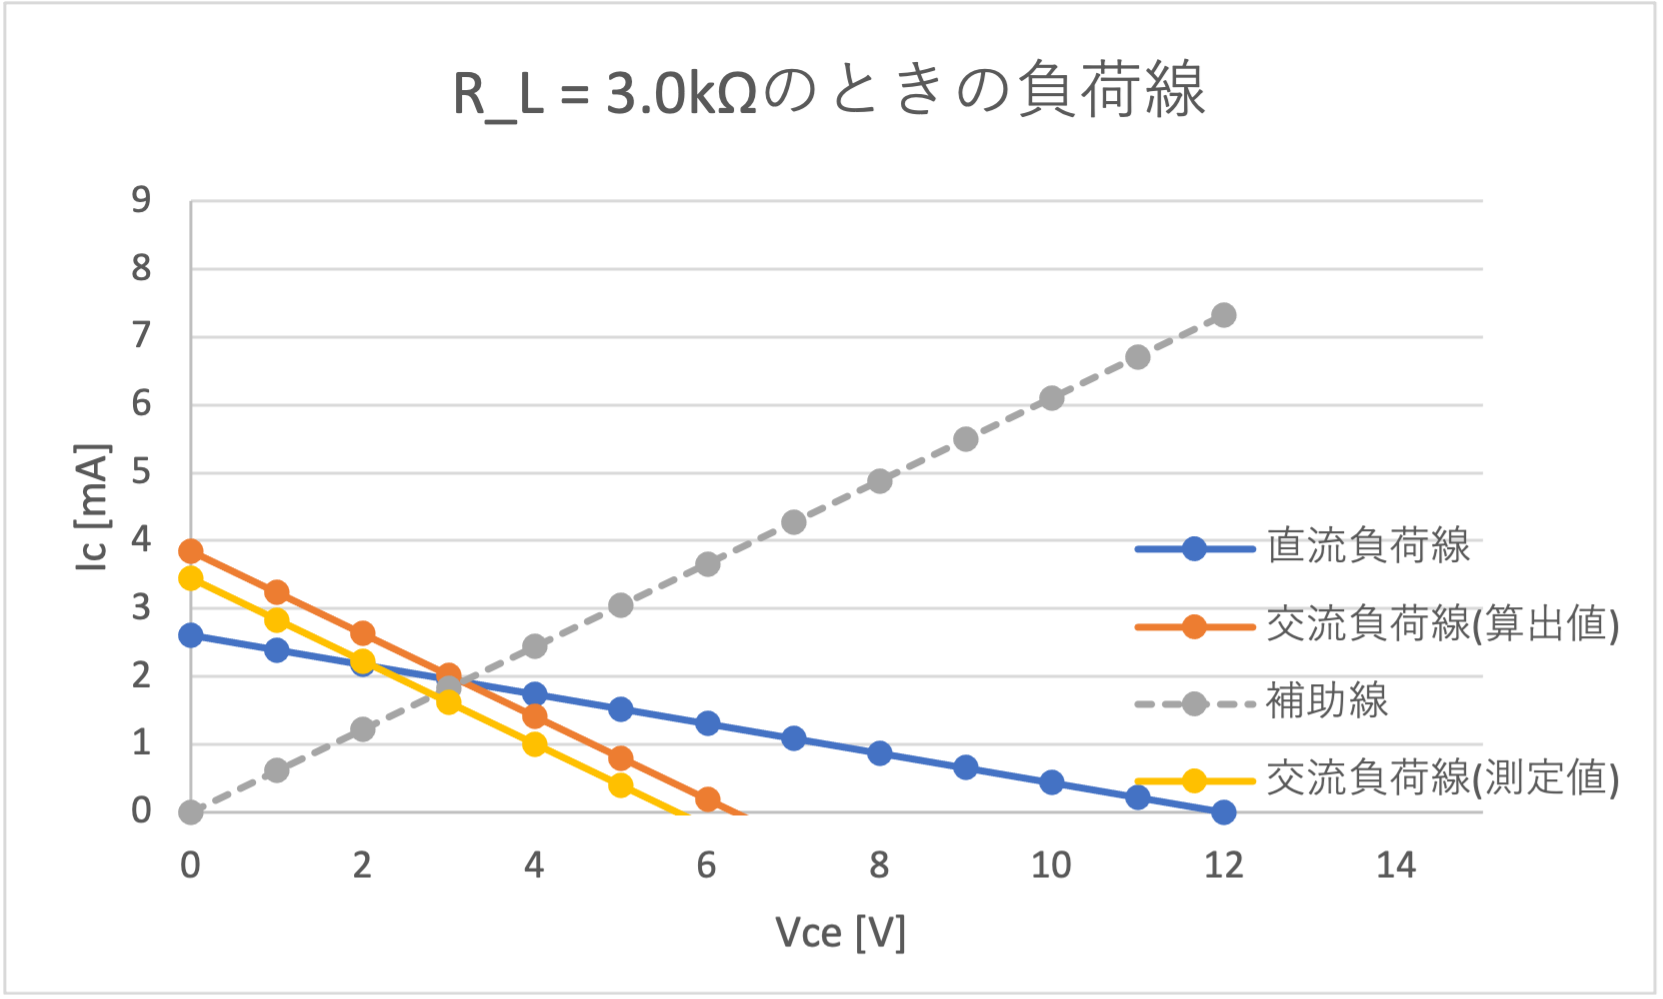
\includegraphics[clip,width=7.5cm]{picture/G3.png}
    \end{center}
    \subcaption{$R_L=3\si{\kilo \ohm}$のときの負荷線}
    \label{G:3huka}
  \end{minipage}
  \caption{負荷線}
  \label{G:hukasen}
\end{figure}\par
交流負荷線を見ると,図\ref{G:1_5huka},\ref{G:3huka}どちらも,算出値と測定値の負荷線が
ずれており,これは動作点が算出値と比べてずれていることを意味する.算出値の出力波形は歪んでいないもの
と考えると,動作点がずれることで,出力波形の片側が歪んでくるとこが予想できる.
この現象について更に考察すると,入力電圧が正の半坡のとき,バイアス電流$I_b$に入力電流$i_v$が加わる.
よって,ベース電流$i_b$が増加し,それに伴いコレクタ電流が増える.ここで,コレクタ電圧は,$V_C=V_{CC}-I_C\times R_c$で
表すことができ,コレクタ電流が増えるとコレクタ電圧は減る.ただし,コレクタ電圧はグランドより下がることはないため,0に出力波形
が近づくとそれ以上は下がらず歪んだ形が出力される.~\cite{uni}

\section{感想}
図\ref{G:result}を見ると,グラフの一部に凸部が見られる.これらの値を理論値と比べて考えると,
値の取り間違い(ヒューマンエラー)だと予想できた.これらは値の書き間違いから発生しており,値を取りながらの
確認が不十分であったことが原因である.ヒューマンエラーにより実験結果に大きな影響がでてきてしまうことがわかったため,
今後はグラフ化しながら実験データを取得するなどして,視覚的にわかりやすい確認を随時行うことが大切であると今回の実験でわかった.

\begin{thebibliography}{99}
  \bibitem{text} 西村壮平: ''トランジスタ基本増幅回路の設計'' (最終閲覧日 2021年6月29日)
  \bibitem{uni} UNICRAFT: ''シミュレーション 低周波増幅回路,波形のひずみ,回路増幅度'' P6 (最終閲覧日 2021年7月4日) \\ \url{http://www.unicraft.co.jp/_files/simulation/FixedBiasAmplifier.pdf}

\end{thebibliography}

\end{document}